\usetikzlibrary{calc}
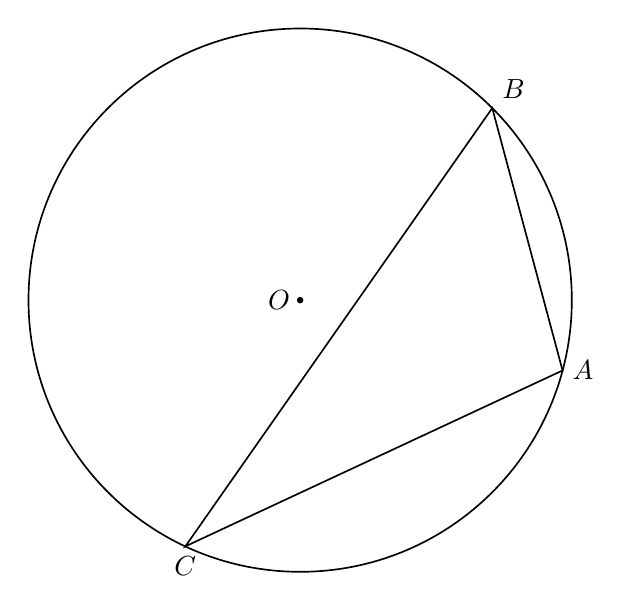
\begin{tikzpicture}[x=1cm,y=1cm,line width=.6pt,font=\normalsize]
\coordinate (O) at (0,0);
\coordinate (A) at (3.3325,-0.893);
\coordinate (B) at (2.4395,2.4395);
\coordinate (C) at (-1.4581,-3.1267);
\draw[black] (O) circle[radius=3.45cm];
\fill[black] (O) circle[radius=1.2pt];
\draw[black] (A)--(B)--(C)--cycle;
\node[left] at (O) {$O$};
\node[right] at (A) {$A$};
\node[above right] at (B) {$B$};
\node[below] at (C) {$C$};
\end{tikzpicture}
